\newpage
\section{Задание 2}

\subsection*{Постановка задачи}

Вычисление скорости Wi-Fi соединений.

\begin{figure}[H]
    \centering
    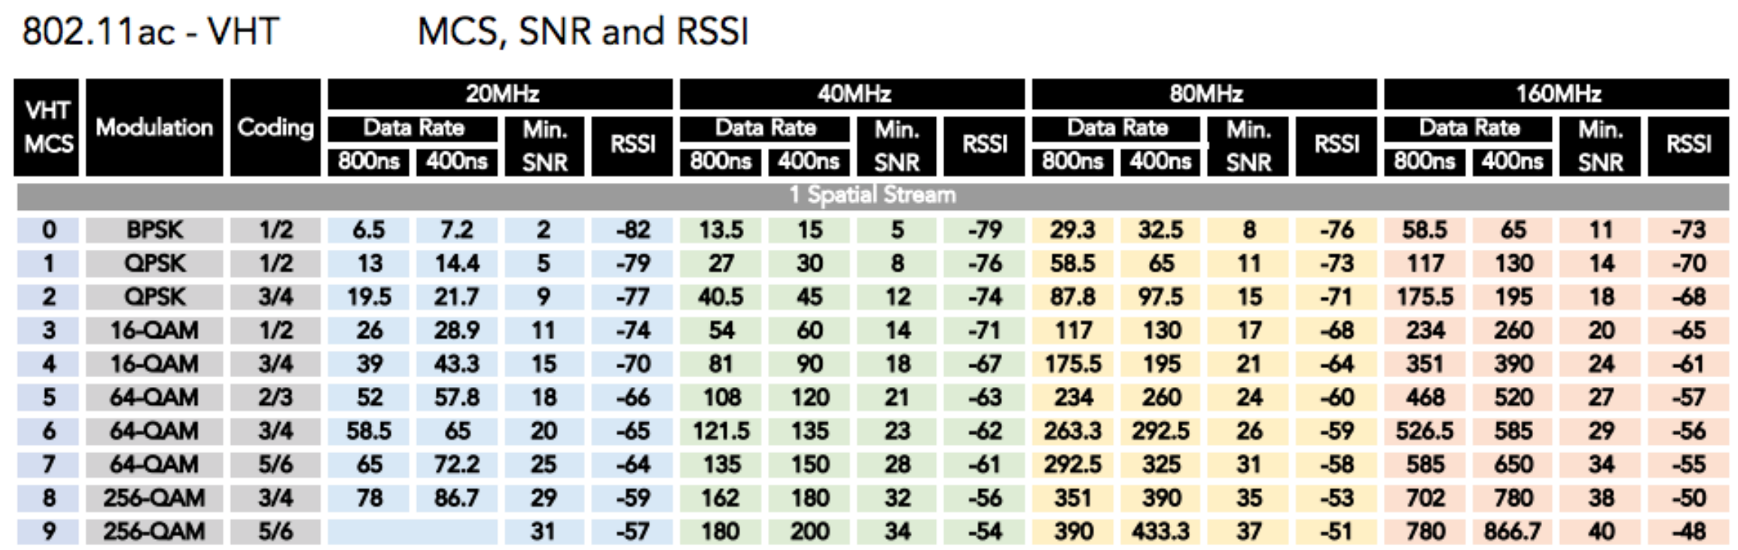
\includegraphics[width=\textwidth]{images/task2.png}
    \caption{Таблица MCS, SNR и RSSI для 802.11ac}
    \label{fig:task2}
\end{figure}

Используя представленную таблицу, необходимо вычислить MCS, модуляцию
и соотношение скоростей соединения Wi-Fi для двух устройств.

Два устройства (A и B) подключены к одному роутеру 802.11ac.
Параметры соединения (ширина канала и количество пространственных
потоков) выбираются с учетом наименьших значений, допустимых для
данной силы сигнала.

\begin{table}[H]
\centering
\begin{tabular}{|l|c|c|}
\hline
\textbf{Параметр соединения} &
\textbf{Устройство A} &
\textbf{Устройство B} \\ \hline

\textbf{Сила сигнала (RSSI)} &
\texttt{-56 dBm} &
\texttt{-67,5 dBm} \\ \hline

\textbf{Макс. ширина канала} &
40 МГц &
80 МГц \\ \hline

\textbf{Конфигурация MIMO} &
2 (MIMO 2$\times$2) &
4 (MIMO 4$\times$4) \\ \hline

\end{tabular}
\caption{Параметры соединения устройств A и B с роутером 802.11ac (вариант 22)}
\label{tab:wifi_devices_22}
\end{table}

\subsection*{Ход выполнения}

Для определения MCS используется таблица, представленная на
рисунке~\ref{fig:task2}. Для каждого устройства необходимо найти
максимальный MCS, при котором фактический уровень RSSI не ниже
требуемого значения, указанного в таблице для соответствующей ширины
канала.

Для устройства A:

\[
RSSI_A=-56\text{ dBm}
\]

При ширине канала 40 МГц для MCS 9 требуется RSSI не менее
$-54$ dBm. Поскольку

\[
-56 < -54,
\]

MCS 9 использовать нельзя.

Для MCS 8 требуется RSSI $-56$ dBm. В этом случае:

\[
-56 \geq -56.
\]

Следовательно,

\[
\boxed{MCS_A=8}
\]

Для MCS 8 используется модуляция 256-QAM и скорость кодирования
$3/4$.

Для одного пространственного потока при ширине канала 40 МГц
скорость составляет 162 Мбит/с при GI = 800 ns и 180 Мбит/с
при GI = 400 ns.

Так как устройство A использует 2 пространственных потока:

\[
R_{A,800}=162\cdot2=324\text{ Мбит/с},
\]

\[
R_{A,400}=180\cdot2=360\text{ Мбит/с}.
\]

Для устройства B:

\[
RSSI_B=-67{,}5\text{ dBm}.
\]

При ширине канала 80 МГц для MCS 4 требуется RSSI не менее
$-64$ dBm. Поскольку

\[
-67{,}5 < -67,
\]

MCS 4 использовать нельзя.

Для MCS 3 требуется RSSI $-71$ dBm. В этом случае:

\[
-67{,}5 \geq -71.
\]

Следовательно,

\[
\boxed{MCS_B=3}
\]

Для MCS 3 используется модуляция 16-QAM и скорость кодирования
$1/2$.

Для одного пространственного потока при ширине канала 40 МГц
скорость составляет 54 Мбит/с при GI = 800 ns и 60 Мбит/с
при GI = 400 ns.

Так как устройство B использует 4 пространственных потока:

\[
R_{B,800}=54\cdot4=216\text{ Мбит/с},
\]

\[
R_{B,400}=60\cdot4=240\text{ Мбит/с}.
\]

Полученные результаты представлены в таблице~\ref{tab:wifi_rates_comparison}.

\begin{table}[H]
\centering
\begin{tabular}{|l|c|c|}
\hline
\textbf{Параметр} &
\textbf{Устройство A} &
\textbf{Устройство B} \\ \hline

RSSI &
\texttt{-56 dBm} &
\texttt{-67,5 dBm} \\ \hline

Ширина канала &
40 МГц &
40 МГц \\ \hline

MIMO &
2 &
4 \\ \hline

MCS &
\textbf{8} &
\textbf{3} \\ \hline

Модуляция &
\textbf{256-QAM} &
\textbf{16-QAM} \\ \hline

Coding &
3/4 &
1/2 \\ \hline

1 поток, 800 ns &
162 Мбит/с &
54 Мбит/с \\ \hline

1 поток, 400 ns &
180 Мбит/с &
60 Мбит/с \\ \hline

Итог, 800 ns &
\textbf{324 Мбит/с} &
\textbf{216 Мбит/с} \\ \hline

Итог, 400 ns &
\textbf{360 Мбит/с} &
\textbf{240 Мбит/с} \\ \hline

\end{tabular}
\caption{Сравнительные характеристики и расчетные скорости соединений устройств A и B}
\label{tab:wifi_rates_comparison}
\end{table}

\subsection*{Сравнение устройств}

При GI = 800 ns получены следующие скорости:

\[
R_A=324\text{ Мбит/с}, \qquad
R_B=216\text{ Мбит/с}.
\]

Отношение скоростей составляет:

\[
\frac{R_A}{R_B}
=
\frac{324}{216}=1{,}5.
\]

Следовательно, при GI = 800 ns скорость соединения устройства A в 1,5 раза выше скорости устройства B.

При GI = 400 ns:

\[
R_A=360\text{ Мбит/с}, \qquad
R_B=240\text{ Мбит/с}.
\]

Отношение скоростей:

\[
\frac{R_A}{R_B}
=
\frac{360}{240}=1{,}5.
\]

Таким образом, при обоих значениях защитного интервала соотношение
скоростей практически одинаково:

\[
\boxed{R_A:R_B=1{,}5:1}
\]

Несмотря на большее количество пространственных потоков MIMO у устройства B
(4 против 2), оно обеспечивает более низкую скорость соединения.
Это связано с более низким уровнем сигнала ($-67{,}5$ dBm против $-56$ dBm),
что приводит к использованию более низкого MCS и менее эффективной
модуляции (16-QAM против 256-QAM). В результате скорость устройства A
в 1,5 раза выше скорости устройства B.